\section{Elaborazione di Segnali Digitali (DSP)}
Questa branca della teoria dei segnali si occupa della conversione dal mondo analogico a digitale e viceversa
e sull'elaborazione numerica dei segnali digitali. Questa branca è nata e si è sviluppata molto rapidamente perchè
permette molto facilmente di manipolare i segnali come se fossero numeri, mentre con i circuiti analogici tutto ciò
richiedeva uno sforzo concettuale e costi davvero elevati.
\subsection{Conversione Analogico/Digitale}
Il primo passo per entrare nel mondo digitale è definire la conversione di un segnale reale in discreto ma incontriamo 2 grandi \textbf{ostacoli}:
\begin{itemize}
    \item \textbf{Istanti Infiniti}: se volessimo rendere digitale un segnale $s(t), t \in \mathbb{R}$, ci accorgeremmo che questo
    trasporta informazione infinita, poichè il numero di istanti $t_i$ in un intervallo $\left[t_{min},t_{max} \right]$ è \textbf{denso}. Dunque 
    il primo passo per ottenere un segnale digitale è \textbf{Campionare}
    \item \textbf{Ampiezze Infinite}: anche se riuscissimo a confinare il segnale entro un intervallo limite di ampiezze, il numero di ampiezze
    disponibili sarebbe comunque infinito. Per questo motivo dovremo discretizzare anche il dominio delle ampiezze $Q = \{q_1,q_2,\dots,q_m\}$ detto \textbf{dizionario di quantizzazione}
\end{itemize}
Possiamo riassumere il processo di conversione nella seguente maniera:
\begin{center}
    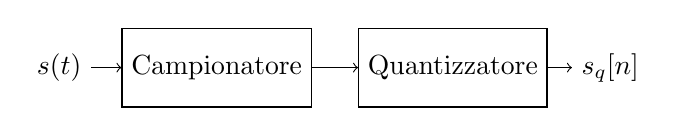
\begin{tikzpicture}
        % Nodo input
        \node at (-2, 0) (input) {$s(t)$};

        % Rettangolo campionatore
        \node[draw, rectangle, minimum width=2cm, minimum height=1cm, align=center] at (0, 0) (sampler) {Campionatore} ;

        % Rettangolo quantizzatore
        \node[draw, rectangle, minimum width=2cm, minimum height=1cm, align=center] at (3, 0) (quantizer) {Quantizzatore};

        % Output
        \node at (5, 0) (output) {$s_q[n]$};

        % Frecce
        \draw[->] (input) -- (sampler) node[midway, above] {};
        \draw[->] (sampler) -- (quantizer) node[midway, above] {};
        \draw[->] (quantizer) -- (output);
    \end{tikzpicture}
\end{center}
E matematicamente ciò corrisponde a:
\begin{center}
    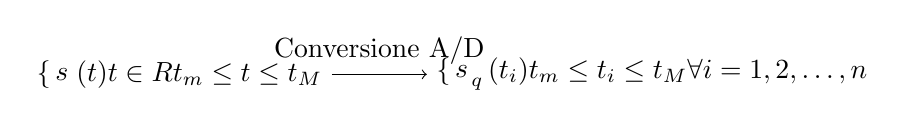
\begin{tikzpicture}
        % Nodo input
        \node at (-3, 0) (input) {
            $\begin{cases}
                s(t)\\
                t \in \mathbb{R}\\
                t_m \leq t \leq t_M
            \end{cases}$
        };

        \node at (3,0) (discr) {
            $
                \begin{cases}
                    s_q(t_i)\\
                    t_m \leq t_i \leq t_M\\
                    \forall i = 1,2,\dots,n
                \end{cases}
            $
        };

        % Frecce
        \draw[->] (input) -- (discr) node[midway, above] {Conversione A/D};
        
    \end{tikzpicture}
\end{center}

\subsection{Campionamento (Sampling)}
Campionare significa registrare, di infiniti istanti, solo di un segnale di alcuni istanti. In generale a noi
interessa campionare il segnale per passi costanti di tempo $T_S$ detto \textbf{Periodo di Campionamento}. Questa
tecnica viene detta \textbf{Campionamento Uniforme} e possiamo formalizzarlo così:
\begin{equation*}
    s(t), t \in \mathbb{R} \longrightarrow s(nT_S) = s_n
\end{equation*}
Dove $n \in \mathbb{Z}$ rappresenta l'i-esimo istante.


    \begin{center}
    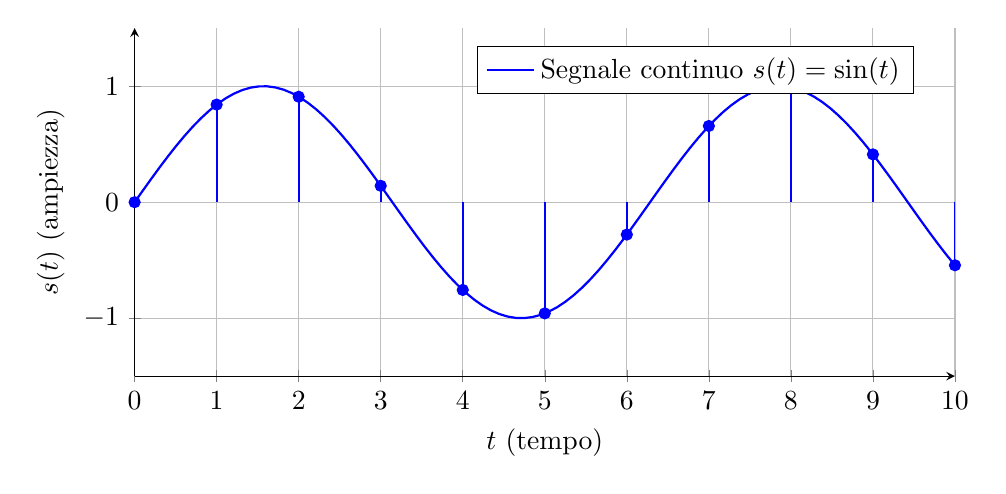
\begin{tikzpicture}
        \begin{axis}[
            width=12cm, height=6cm,
            xlabel={$t$ (tempo)},
            ylabel={$s(t)$ (ampiezza)},
            xmin=0, xmax=10,
            ymin=-1.5, ymax=1.5,
            xtick={0,1,2,3,4,5,6,7,8,9,10},
            ytick={-1,0,1},
            grid=both,
            domain=0:10,
            samples=100,
            axis lines=left,
            legend style={at={(0.95,0.95)}, anchor=north east}
        ]
        
        % Segnale continuo s(t) = sin(t)
        \addplot[blue, thick] {sin(deg(x))};
        \addlegendentry{Segnale continuo $s(t) = \sin(t)$}
        
        % Campionamento del segnale con bastoncini e punti campionati
        \foreach \x in {0,1,2,3,4,5,6,7,8,9,10} {
            \pgfmathsetmacro{\y}{sin(deg(\x))} % Calcolo del valore y = sin(x)
            
            % Punto campionato
            \addplot[blue, mark=*, only marks, mark options={fill=blue}] coordinates {(\x,\y)};
            \addplot[blue, thick] coordinates {(\x,0) (\x,\y)};
        }
        
    \end{axis}
    \end{tikzpicture}
\end{center}

Dal grafico possiamo riconoscere come questi siano tanti impulsi di Dirac, ognuno traslato di un certo $nT_S$ e 
con una determinata ampiezza: 
\begin{equation}
    \delta_{T_S} (t) = \sum_{-\infty}^{+\infty} \delta (t - nT_S)
\end{equation}
Grazie a ciò possiamo definire il \textbf{Campionamento Ideale}:
\begin{align*}
    s_c(t) &= s(t) \cdot \delta_{T_S} (t) =\\ 
           &= s(t)\sum_{-\infty}^{+\infty} \delta (t - nT_S) = \\
           &= \sum_{-\infty}^{+\infty} s(nT_S) \delta (t - nT_S)
\end{align*}
Nella realtà, tuttavia, un campionamento del genere non è possibile (non è possibile proprio generare un impulso di dirac)
queste formalizzazioni tuttavia servono per permetterci di studiare meglio i segnali digitali.
\subsection{Spettro del Segnale Campionato}
Grazie alla formalizzazione precedente possiamo determinare lo spettro del segnale $s_c(t)$, ossia:
\begin{equation}
    s_c(t) = s(t)\delta_{T_S}(t) \fCouple S(f)\ast\Delta_{T_S}(f) = S_c(f)
\end{equation}
Dal momento che $\delta_{T_S}(t)$ possiamo vederla come una funzione periodica di periodo $T_S$, allora possiamo esprimere
la funzione tramite lo \textbf{sviluppo in serie di fourier}:
\begin{equation}
    \delta_{T_S}(t) = \sum_{n = -\infty}^{+\infty} c_n e^{j2\pi\frac{n}{Ts}t}
\end{equation}
Calcoliamoci dunque $c_n$:
\begin{align*}
    c_n &= \frac{1}{T_S}\int_{-\frac{T}{2}}^{\frac{T}{2}} \delta_{T_S}(t)e^{-j2\pi \frac{n}{Ts}t}dt=\\
        &= \frac{1}{T_S}\int_{-\frac{T}{2}}^{\frac{T}{2}} \delta(t)e^{-j2\pi \frac{n}{Ts}t}dt=\\
        &= \frac{1}{T_S}e^{-j0} \tag{per il campionamento}
\end{align*}
Possiamo dunque notare come i coefficienti dello sviluppo in serie siano tutti $\frac{1}{T_S}$, ossia:
\begin{equation}
    \delta_{T_S}(t) = \frac{1}{T_S}\sum_{n = -\infty}^{+\infty} e^{j2\pi\frac{n}{Ts}t}
\end{equation}